\chapter{Introduction} \label{ch:intro}

% Subject matter terms are addressed with \texttt{\textbackslash gls\{glossary-label\}} like so \gls{glossary-label}. \\
% Acronyms are addressed with either with their long equivalent \texttt{\textbackslash acrlong\{gls-label\}} which gives \acrlong{acronym-label}
% or the short equivalent \texttt{\textbackslash acrshort\{gls-label\}} which gives \acrshort{acronym-label}. \\
% Subject matter terms can also be multi structure \texttt{\textbackslash gls\{glossary-multi-label\}} which gives \gls{glossary-multi-label} (see terms and acronyms above). \medskip

The developments in robotics as a field has over the past years provided automation solutions to execute repetitive manual tasks with high efficiency and reliability \fakecite. One of the most common tasks being pick and place tasks which involves picking un an object from one position and placing is in another. This is can be parted into the following subparts: Object localization, pose estimation, grasping and placing. In the solutions currently present for industrial use \gls{cv} is used for object localization and \gls{pe} due to the low cost of cameras and the fields maturity. However, while these solutions may be sufficient for certain tasks they fundamentally suffer from the weaknesses introduced by vision techniques. These include a great number of outliers caused by occlusions, reflecting, transparent or homogeneous surfaces, and repetitive structures when solving the \gls{corr-problem}. These problems as of the writing of this project have jet to be completely solved. Promising results have been found with the rise of \gls{dl} which in present time has proven its versatility and provides proof of concept solutions for narrow cases in pose estimation of transparent \cite{6dof-pose-estimation-of-transparent-object-from-a-single-rgb-d-image} and reflective objects \cite{6d-pose-estimation-of-objects:-recent-technologies-and-challenges}. This is relevant since industrial settings often contain transparent and especially reflecting objects as metallic parts tend to appear frequently and have high reflectances. \medskip

\begin{minipage}{0.45\textwidth}
	To solve these problems this project aims to perform in-hand pose estimation through only the use of tactile sensors. Specifically this will be done on a Shadow Dexterous Hand \cite{shadow-dex-hand} with 20 \gls{dof}. Using tactile inputs rather than visual, eliminates the weaknesses mentioned above. A schematic showing the hand can be seen in \figref{fig:shadow-dex-hand-schematic}. Using this approach, the overall problem can be partitioned into 3 sub-problems labeled problem 1, 2 and 3. Problem 1 involves modeling the contact between the gripper's fingers and the object, also referred to as tactile perception. Problem 2 is to convert the collected data from problem 1 to meaningful surface data, treat these data as features and use them to estimate pose candidates. Finally problem 3 involves in-hand manipulation, such that further information is gained by probing the object. Here new desired surface points are found such that strong surface features are found to better identify the object's correct pose. 
	The development of this project is done in the \gls{docker} provided by Shadow Robotics for simulation, control and development of the hand \cite{shadow-dex-github}. Here a hardware-simulation agnostic \gls{ros} \cite{ros} control \cite{ros-control} interface is provided, which provides fundamental tools to interact with the robot hand. \medskip
	\end{minipage} 
	\hfill
	\begin{minipage}{0.45\textwidth}
	\begin{figure}[H]
		\begin{small}
			\begin{center}
				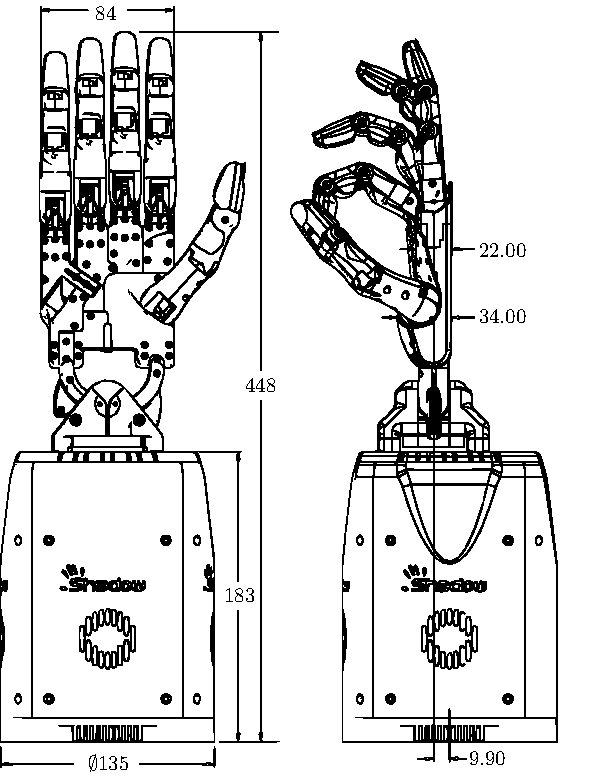
\includegraphics[width=0.95\textwidth]{chapters/introduction/fig/shadow-dex-hand-vector.pdf}
			\end{center}
			\caption{Schematic of Shadow Dexterous Hand from Shadow Robots, based on \cite{shadow-dex-hand-schematic}. The measurements are in \SI{}{\milli\metre}.}
			\label{fig:shadow-dex-hand-schematic}
		\end{small}
	\end{figure}
\end{minipage}

The dynamic simulation environment Gazebo \cite{gazebo} is provided as part of the \gls{docker} and is thus the one used for this project. \medskip
To solve the problems presented \gls{ros} packages are developed with the \tabref{tab:software-package-table}


\begin{table}
	\begin{small}
		\begin{center}
			\begin{tabular}[c]{ | l r | l | } \hline
				\cellcolor{tableheader} \textbf{Package}           & \cellcolor{tableheader} & \multicolumn{1}{l|}{\cellcolor{tableheader} \textbf{Description}} \\ \hline \hline
				\texttt{in\_hand\_pose\_estimation}                & \meta{meta} & \textbf{Project package of the in-hand pose estimation system} \\ \hline
				\hspace{0.3cm} \texttt{in\_hand\_pose\_estimation} &             & Integration of the full in-hand pose estimation pipeline  \\ \hline
				\hspace{0.3cm} \texttt{sr\_tactile\_image}         & \pkg{pkg}   & Extraction of tactile perception  \\ \hline
				\hspace{0.3cm} \texttt{sr\_pose\_estiamtion}       & \pkg{pkg}   & Estimate the pose of object based on tactile perception \\ \hline
				\hspace{0.3cm} \texttt{sr\_hand\_manipulation}     & \pkg{pkg}   & Manipulate object in hand to probe for strong features \\ \hline \hline
				\texttt{sr\_common}                                & \meta{meta} & \textbf{Shadow package for commonly used tools} \\ \hline
				\hspace{0.3cm} \texttt{sr\_common}                 &             & Implements commonly used tools such as messages \\ \hline
				\hspace{0.3cm} \texttt{sr\_robot\_msgs}            & \pkg{pkg}   & Messages used to communicate with the robot hand  \\ \hline 
				\hspace{0.3cm} \texttt{\dots}                      &             &  \\ \hline \hline
				\texttt{sr\_core}                                  & \meta{meta} & \textbf{Shadow package for core tools} \\ \hline
				\hspace{0.3cm} \texttt{sr\_core}                   &             & Implements core features of the hand such as hardware interfacing \\ \hline
				\hspace{0.3cm} \texttt{sr\_hand}                   & \pkg{pkg}   & Contains the hand commander for controlling the robot hand  \\ \hline
				\hspace{0.3cm} \texttt{\dots}                      &             &  \\ \hline \hline
				\texttt{ros\_utils}                                              & \pkg{pkg} & \textbf{Utilities for interfacing ROS/Gazebo/MoveIt/Eigen etc} \\ \hline
			\end{tabular}
		\end{center}
		\caption{Software packages of the in hand pose estimation system.}
		\label{tab:software-package-table}
	\end{small}
\end{table}




{\fontfamily{cmr}\selectfont 
Text in Times%
}

\begin{itemize}
	\item work will be done in simulation provided by shadow robotics\fakecite. ROS, Gazebo, docker.
	\item The project will be implemented as a meta-package with sub packages for each of the problems.
	\item state of the art will be presented in chapter x
\end{itemize}

% o Background information - Helicopter perspective, what is the project all about? Give the outside reader at chance to understand the domain.
% o Problem statement - Wherein lies the problem? What will you try to solve?
o Related work - During your literature search what did you find? - Your own or the research group's prior work if any?
o Project aim or Hypothesis - How did you derive your project aim (engineering design process) or hypothesis which you are testing (scientific method) and how it connects to related work?

% Robot engineering replacing manual labor\\
% Manual labor of different industries (farming, health, transport), focus on Factory work \\
% Bin picking as a generic problem and its sub parts \\
% Current solutions, their parts with pros and cons (localization, pose estimation, grasping, placing) (deeplearning on transparent objects) \\
% How is this project going to solve the problems present in the current solutions \\
% What problems are going to be addressed, how are they going to be addressed and what is the solution's subparts \\
